\chapter{OTA - Exercício 4 - Analíticos} \label{Chap:AppendixAnaliticosA04}

%CASO 1
\begin{xltabular}{\textwidth}{|l|X|X|}
	\hline
	\endfirsthead
	
	\hline \multicolumn{3}{|c|}{continuação da página anterior} \\ \hline
	\endhead
	
	\hline \multicolumn{3}{|r|}{Continua na próxima página} \\ \hline
	\endfoot
	
	\hline
	\endlastfoot
	
	\multicolumn{3}{|c|}{\cellcolor[HTML]{C0C0C0}\textbf{CASO DE TESTE 1}} \\ \hline


%	\multicolumn{3}{|c|}{\cellcolor[HTML]{DEDEDE}\textbf{Nota Ponderada - EF1}} \\ \hline
	\multicolumn{3}{|c|}{\textbf{Blocos}} \\ \hline
	\multicolumn{3}{|l|}{\begin{tabular}[c]{@{}l@{}} \\ 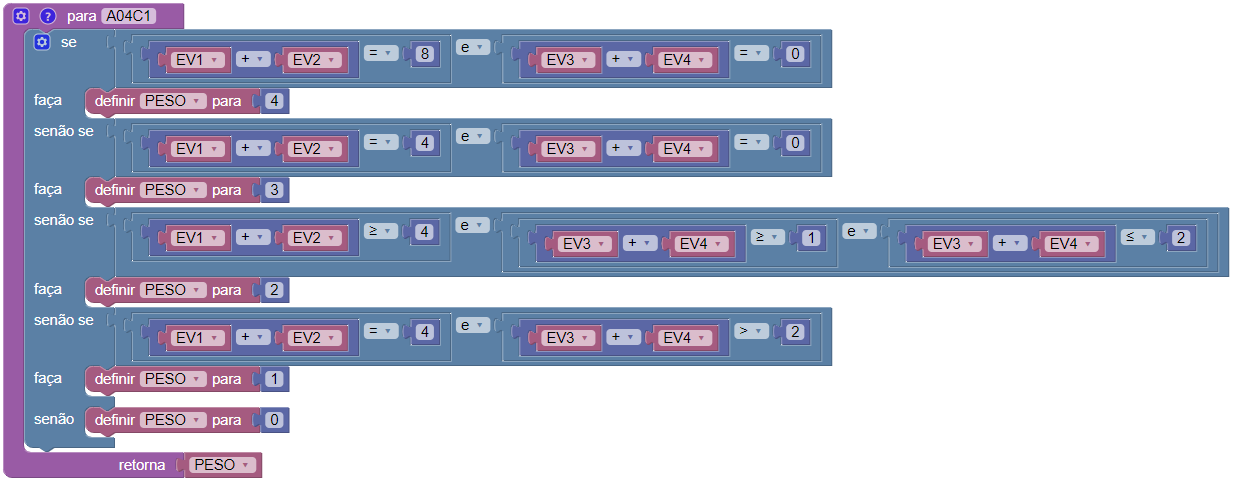
\includegraphics[width=0.9\linewidth]{chapters/appendixAnalytics/A04/C1.png}  \end{tabular}
	} \\ \hline
	\multicolumn{3}{|c|}{\textbf{Python gerado}} \\ \hline
	\multicolumn{3}{|l|}{ \begin{tabular}[c]{@{}l@{}}def A04C1():\\ \quad global PESO, EV1, EV2, EV3, EV4\\ \quad if EV1 + EV2 == 8 and EV3 + EV4 == 0:\\ \qquad PESO = 4\\ \quad elif EV1 + EV2 == 4 and EV3 + EV4 == 0:\\ \qquad PESO = 3\\ \quad elif EV1 + EV2 >= 4 and EV3 + EV4 >= 1 and EV3 + EV4 <= 2:\\ \qquad PESO = 2\\ \quad elif EV1 + EV2 == 4 and EV3 + EV4 > 2:\\ \qquad PESO = 1\\ \quad else:\\ \qquad PESO = 0\\ \quad return PESO\end{tabular} }\\ \hline
	
\end{xltabular}

\pagebreak

%CASO 2
\begin{xltabular}{\textwidth}{|l|X|X|}
	\hline
	\endfirsthead
	
	\hline \multicolumn{3}{|c|}{continuação da página anterior} \\ \hline
	\endhead
	
	\hline \multicolumn{3}{|r|}{Continua na próxima página} \\ \hline
	\endfoot
	
	\hline
	\endlastfoot
	
	\multicolumn{3}{|c|}{\cellcolor[HTML]{C0C0C0}\textbf{CASO DE TESTE 2}} \\ \hline
	
%	\multicolumn{3}{|c|}{\cellcolor[HTML]{DEDEDE}\textbf{Nota Ponderada - EF1}} \\ \hline
	\multicolumn{3}{|c|}{\textbf{Blocos}} \\ \hline
	\multicolumn{3}{|l|}{\begin{tabular}[c]{@{}l@{}} \\ 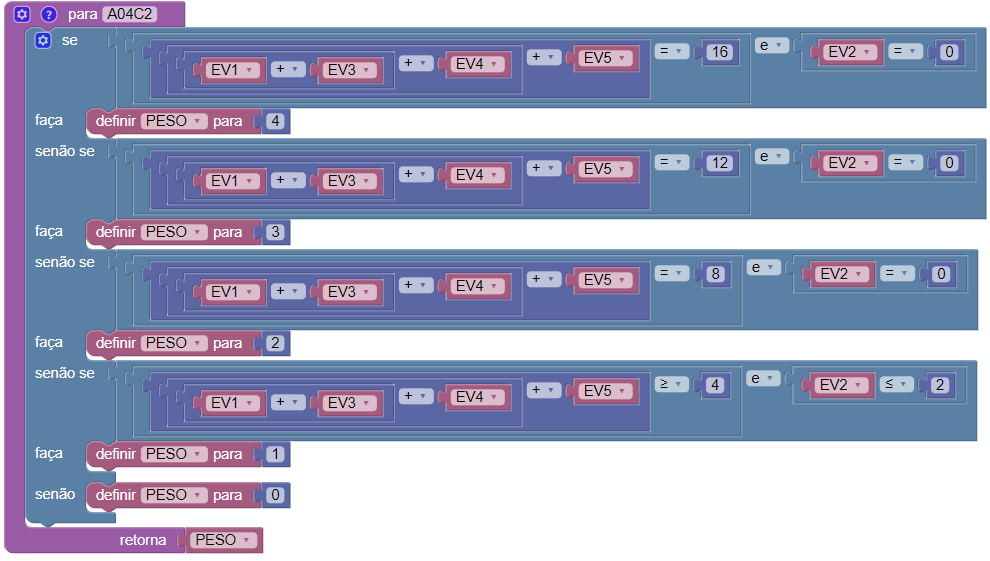
\includegraphics[width=0.9\linewidth]{chapters/appendixAnalytics/A04/C2.png}  \end{tabular}
	} \\ \hline
	\multicolumn{3}{|c|}{\textbf{Python gerado}} \\ \hline
	\multicolumn{3}{|l|}{ \begin{tabular}[c]{@{}l@{}}def A04C2():\\ \quad global PESO, EV2, EV5, EV4, EV1, EV3\\ \quad if ((EV1 + EV3) + EV4) + EV5 == 16 and EV2 == 0:\\ \qquad PESO = 4\\ \quad elif ((EV1 + EV3) + EV4) + EV5 == 12 and EV2 == 0:\\ \qquad PESO = 3\\ \quad elif ((EV1 + EV3) + EV4) + EV5 == 8 and EV2 == 0:\\ \qquad PESO = 2\\ \quad elif ((EV1 + EV3) + EV4) + EV5 >= 4 and EV2 <= 2:\\ \qquad PESO = 1\\ \quad else:\\ \qquad PESO = 0\\ \quad return PESO \end{tabular} }\\ \hline
	
\end{xltabular}

\pagebreak
%CASO 3
\begin{xltabular}{\textwidth}{|l|X|X|}
	\hline
	\endfirsthead
	
	\hline \multicolumn{3}{|c|}{continuação da página anterior} \\ \hline
	\endhead
	
	\hline \multicolumn{3}{|r|}{Continua na próxima página} \\ \hline
	\endfoot
	
	\hline
	\endlastfoot
	
	\multicolumn{3}{|c|}{\cellcolor[HTML]{C0C0C0}\textbf{CASO DE TESTE 3}} \\ \hline
	
	%EF1
%	\multicolumn{3}{|c|}{\cellcolor[HTML]{DEDEDE}\textbf{Nota Ponderada - EF1}} \\ \hline
	\multicolumn{3}{|c|}{\textbf{Blocos}} \\ \hline
	\multicolumn{3}{|l|}{\begin{tabular}[c]{@{}l@{}} \\ 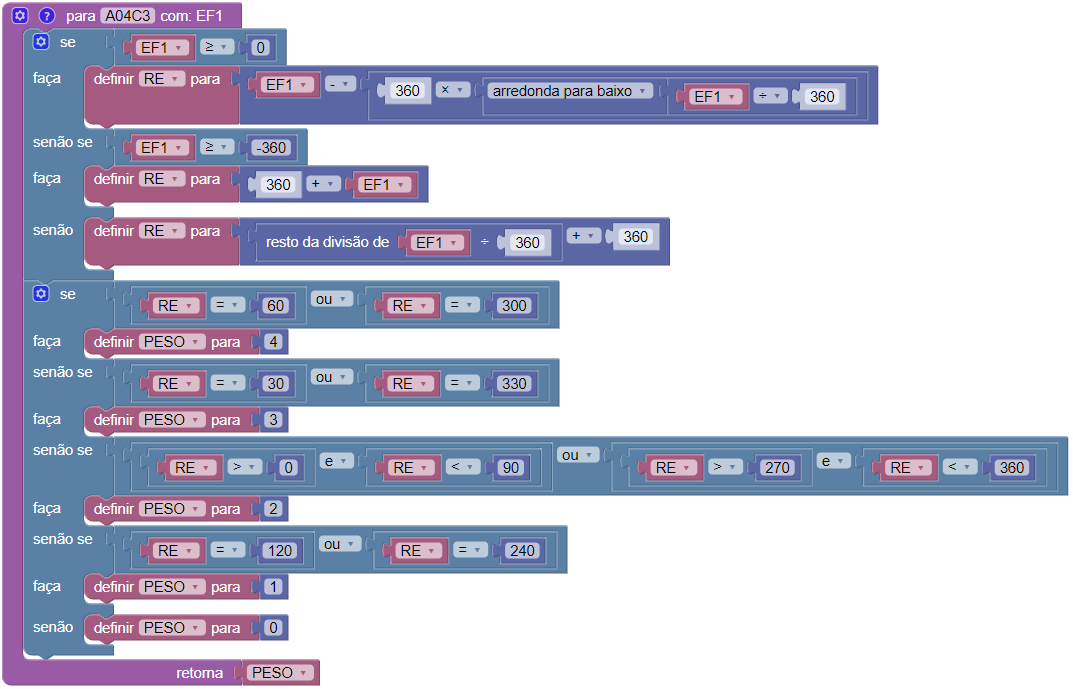
\includegraphics[width=0.9\linewidth]{chapters/appendixAnalytics/A04/C3.png}  \end{tabular}
	} \\ \hline
	\multicolumn{3}{|c|}{\textbf{Python gerado}} \\ \hline
	\multicolumn{3}{|l|}{ \begin{tabular}[c]{@{}l@{}}import math \\ \# Nota Ponderada - EF1 - Caso 3 - A04\\ def A04C3(EF1):\\ \quad global PESO, RE\\ \quad if EF1 >= 0:\\ \qquad RE = EF1 - 360 * math.floor(EF1 / 360)\\ \quad elif EF1 >= -360:\\ \qquad RE = 360 + EF1\\ \quad else:\\ \qquad RE = EF1 \% 360 + 360\\ \quad if RE == 60 or RE == 300:\\ \qquad PESO = 4\\ \quad elif RE == 30 or RE == 330:\\ \qquad PESO = 3\\ \quad elif RE > 0 and RE < 90 or RE > 270 and RE < 360:\\ \qquad PESO = 2\\ \quad elif RE == 120 or RE == 240:\\ \qquad PESO = 1\\ \quad else:\\ \qquad PESO = 0\\ \quad return PESO \end{tabular} }\\ \hline
	
\end{xltabular}

\pagebreak
%CASO 4
\begin{xltabular}{\textwidth}{|l|X|X|}
	\hline
	\endfirsthead
	
	\hline \multicolumn{3}{|c|}{continuação da página anterior} \\ \hline
	\endhead
	
	\hline \multicolumn{3}{|r|}{Continua na próxima página} \\ \hline
	\endfoot
	
	\hline
	\endlastfoot
	
	\multicolumn{3}{|c|}{\cellcolor[HTML]{C0C0C0}\textbf{CASO DE TESTE 4}} \\ \hline
	
	%EF1
%	\multicolumn{3}{|c|}{\cellcolor[HTML]{DEDEDE}\textbf{Nota Ponderada - EF1}} \\ \hline
	\multicolumn{3}{|c|}{\textbf{Blocos}} \\ \hline
	\multicolumn{3}{|l|}{\begin{tabular}[c]{@{}l@{}} \\ 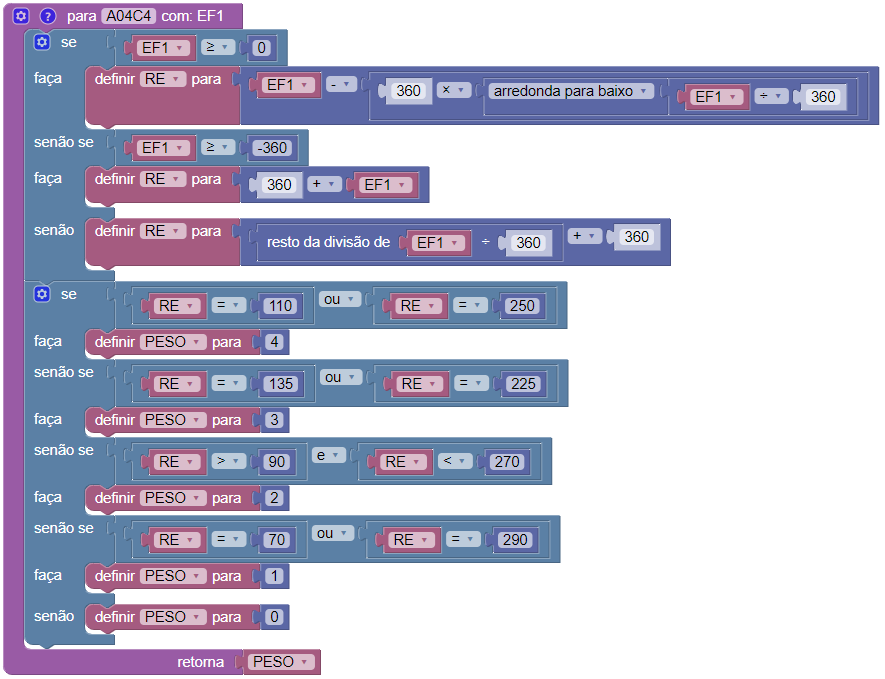
\includegraphics[width=0.9\linewidth]{chapters/appendixAnalytics/A04/C4.png}  \end{tabular}
	} \\ \hline
	\multicolumn{3}{|c|}{\textbf{Python gerado}} \\ \hline
	\multicolumn{3}{|l|}{ \begin{tabular}[c]{@{}l@{}}import math \\ \# Nota Ponderada - EF1 - Caso 4 - A04\\ def A04C4(EF1):\\ \quad global PESO, RE\\ \quad if EF1 >= 0:\\ \qquad RE = EF1 - 360 * math.floor(EF1 / 360)\\ \quad elif EF1 >= -360:\\ \qquad RE = 360 + EF1\\ \quad else:\\ \qquad RE = EF1 \% 360 + 360\\ \quad if RE == 110 or RE == 250:\\ \qquad PESO = 4\\ \quad elif RE == 135 or RE == 225:\\ \qquad PESO = 3\\ \quad elif RE > 90 and RE < 270:\\ \qquad PESO = 2\\ \quad elif RE == 70 or RE == 290:\\ \qquad PESO = 1\\ \quad else:\\ \qquad PESO = 0\\ \quad return PESO \end{tabular} }\\ \hline
	
\end{xltabular}

\pagebreak
%CASO 5
\begin{xltabular}{\textwidth}{|l|X|X|}
	\hline
	\endfirsthead
	
	\hline \multicolumn{3}{|c|}{continuação da página anterior} \\ \hline
	\endhead
	
	\hline \multicolumn{3}{|r|}{Continua na próxima página} \\ \hline
	\endfoot
	
	\hline
	\endlastfoot
	
	\multicolumn{3}{|c|}{\cellcolor[HTML]{C0C0C0}\textbf{CASO DE TESTE 5}} \\ \hline
	
	%EF1
%	\multicolumn{3}{|c|}{\cellcolor[HTML]{DEDEDE}\textbf{Nota Ponderada - EF1}} \\ \hline
	\multicolumn{3}{|c|}{\textbf{Blocos}} \\ \hline
	\multicolumn{3}{|l|}{\begin{tabular}[c]{@{}l@{}} \\ 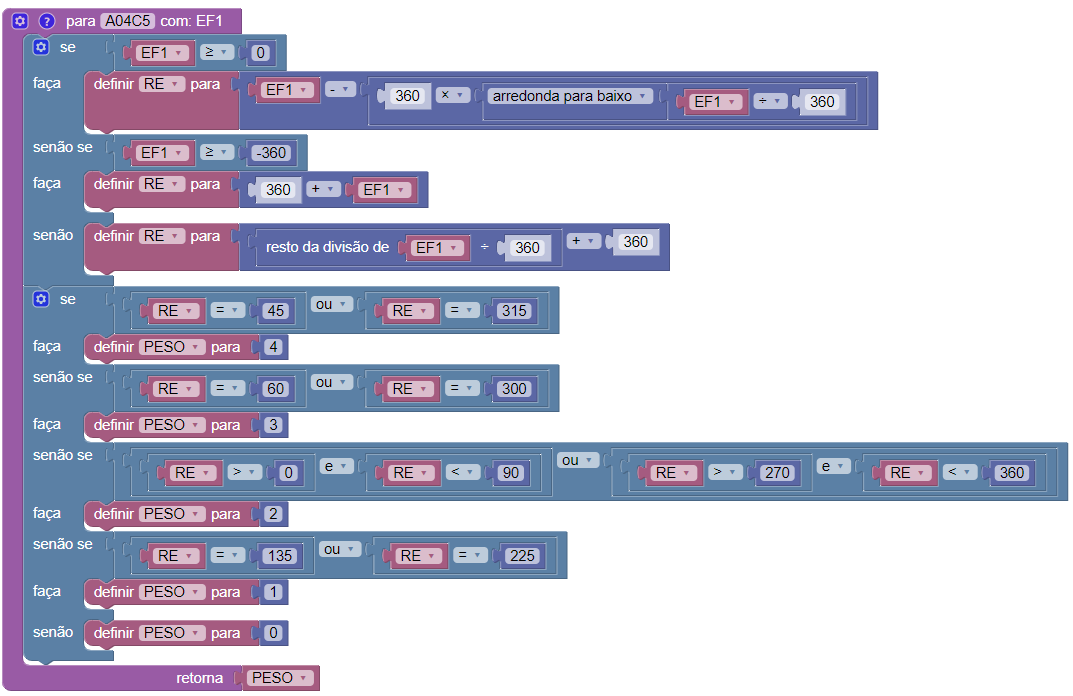
\includegraphics[width=0.9\linewidth]{chapters/appendixAnalytics/A04/C5.png}  \end{tabular}
	} \\ \hline
	\multicolumn{3}{|c|}{\textbf{Python gerado}} \\ \hline
	\multicolumn{3}{|l|}{ \begin{tabular}[c]{@{}l@{}}import math\\ \# Nota Ponderada - EF1 - Caso 5 - A04\\ def A04C5(EF1):\\ \quad global PESO, RE\\ \quad if EF1 >= 0:\\ \qquad RE = EF1 - 360 * math.floor(EF1 / 360)\\ \quad elif EF1 >= -360:\\ \qquad RE = 360 + EF1\\ \quad else:\\ \qquad RE = EF1 \% 360 + 360\\ \quad if RE == 45 or RE == 315:\\ \qquad PESO = 4\\ \quad elif RE == 60 or RE == 300:\\ \qquad PESO = 3\\ \quad elif RE > 0 and RE < 90 or RE > 270 and RE < 360:\\ \qquad PESO = 2\\ \quad elif RE == 135 or RE == 225:\\ \qquad PESO = 1\\ \quad else:\\ \qquad PESO = 0\\ \quad return PESO \end{tabular} }\\ \hline
		
\end{xltabular}

\pagebreak
%CASO 6
\begin{xltabular}{\textwidth}{|l|X|X|}
	\hline
	\endfirsthead
	
	\hline \multicolumn{3}{|c|}{continuação da página anterior} \\ \hline
	\endhead
	
	\hline \multicolumn{3}{|r|}{Continua na próxima página} \\ \hline
	\endfoot
	
	\hline
	\endlastfoot
	
	\multicolumn{3}{|c|}{\cellcolor[HTML]{C0C0C0}\textbf{CASO DE TESTE 6}} \\ \hline
	
	%EF1
%	\multicolumn{3}{|c|}{\cellcolor[HTML]{DEDEDE}\textbf{Nota Ponderada - EF1}} \\ \hline
	\multicolumn{3}{|c|}{\textbf{Blocos}} \\ \hline
	\multicolumn{3}{|l|}{\begin{tabular}[c]{@{}l@{}} \\ 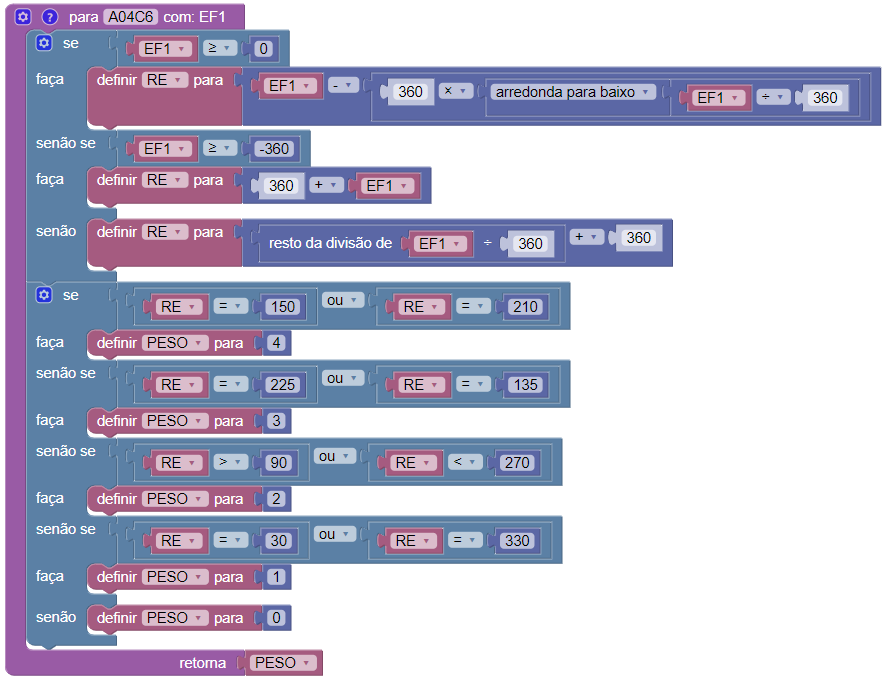
\includegraphics[width=0.9\linewidth]{chapters/appendixAnalytics/A04/C6.png}  \end{tabular}
	} \\ \hline
	\multicolumn{3}{|c|}{\textbf{Python gerado}} \\ \hline
	\multicolumn{3}{|l|}{ \begin{tabular}[c]{@{}l@{}} import math \\ \# Nota Ponderada - EF1 - Caso 6\\ \# Redução ao primeiro quadrante\\ def A04C6(EF1):\\ \quad global PESO, RE\\ \quad if EF1 >= 0:\\ \qquad RE = EF1 - 360 * math.floor(EF1 / 360)\\ \quad elif EF1 >= -360:\\ \qquad RE = 360 + EF1\\ \quad else:\\ \qquad RE = EF1 \% 360 + 360\\ \quad if RE == 150 or RE == 210:\\ \qquad PESO = 4\\ \quad elif RE == 225 or RE == 135:\\ \qquad PESO = 3\\ \quad elif RE > 90 or RE < 270:\\ \qquad PESO = 2\\ \quad elif RE == 30 or RE == 330:\\ \qquad PESO = 1\\ \quad else:\\ \qquad PESO = 0\\ \quad return PESO \end{tabular} }\\ \hline
	
\end{xltabular}

